 \section{Summary}
 With the availability of powerfull hardware as GPUs (Graphics Processing Unit) wich were initialy built for video game and could operate huge mathematical operations quickly, data bank and algorithms, deep learning became very popular.  A lot of graphical user interface for training and developping deep neural network are available. Like Expresso for Caffe, NVidia DIGITS for Theano, Caffe, Torch and Tensorflow. Unfortunately they are not compatible with the PyTorch library at the time when we began this project. The alternative we propose is an application that will be an interface for PyTorch for training and developping deep neural network with the Pytorch framework.

\section{Domain descripton}
Our application is developed for user who want to build/modify neural network model with PyTorch, a recent deep learning framework developed by Facebook since October 2016. Deep Learning algorithms are a part of the machine learning family algorithms. Machine learning is one of the fields of study of Artificial Intelligence. It relies on statistical concepts as well as models to give machines the ability to learn. It basically consists of showing a lots of examples, using a set of data, the training set, to make our algorithm try to recognize patterns in it, so it can learn to recognize new data instantly thus come up with rules to predict outcomes for unseen data:

\begin{figure}[!ht]
    \center
    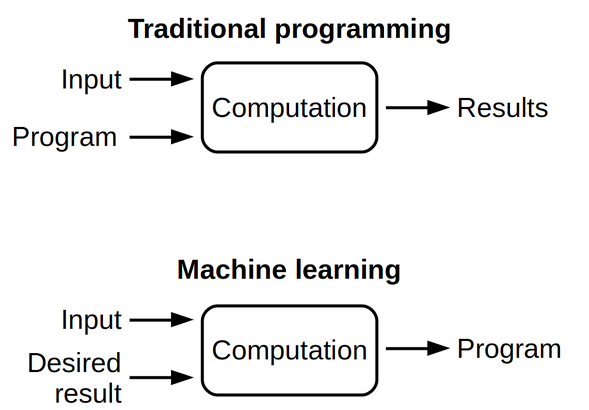
\includegraphics[scale=0.3]{figures/marchine_learning_para.png}
    \caption{Traditional Programming vs Machine Learning}
\end{figure}


The training phase of a machine learning algorithm takes the training set, and tries for a pre-determined number of iterations, to classify the data. In each iteration, the algorithm will take into account the errors of classification in the last iteration to correct itself, step by step, until its accuracy is high enough.

There are different types of approach for machine learning algorithms :
\begin{itemize}
\item Supervised learning : In this case, the data is annotated, which means the algorithm knows the inputs and the outputs of the set. It allows to directly check if the result is correct in each iteration.
\item Semi-supervised learning : In this case it's the same as supervised learning, with the exception that only a part of the data is annotated
\item Unsupervised learning : This type of approach is clearly distinct from the two others, since the data is not annotated. In this case, the algorithm will try to find patterns by itself, without the use of external corrections. It's only after training that the user can see the results.
\end{itemize}

Once the training of the algorithm is finished, we can evaluate it by using another data-set, which contains different data than the training set, to evaluate the accuracy of our algorithm. \usetikzlibrary{}Here is a visualization among AI, ML and DL.

\begin{figure}[!ht]
    \center
    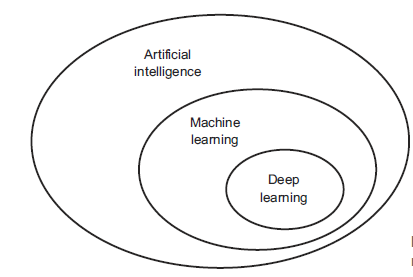
\includegraphics[scale=0.5]{figures/aivsmlvsdl.png}
    \caption{About AI}
\end{figure}

Deep Learning algorithms are a part of the machine learning family algorithms. To be able to recognize patterns in data, they use a cascade of multiple layers of nonlinear processing units. Each layer uses the output from the previous one. They work with the concept of deep neural networks.
\\\
\\\


\subsection{How a computer deals with input data}
When a computer operates on an image, it will obtain an array  of pixel values that the numbers of pixels would depend on the size of image but will have three values or more specifically can say three dimensions. The first and second dimensions are the height and wide of image and the third value will represent the coloring scheme Red, Green, Blue in short RGB.  
For instance, we have a 480 X 480  image,  the  represented  image  will be 480 X 480 X 3. 

Each of these numbers, between 1-480 X 480 (according to our example) is given a value from 0 to 255 which describes the pixels' intensity at that point; means if a pixel color is white, it will has a value which corresponds the white color (more likely zero) and if a pixel color is red, it will has a value corresponded to the red color. The intensity of the all different colors are in the range of 0 to 255.

\begin{figure}[]
    \centering 
    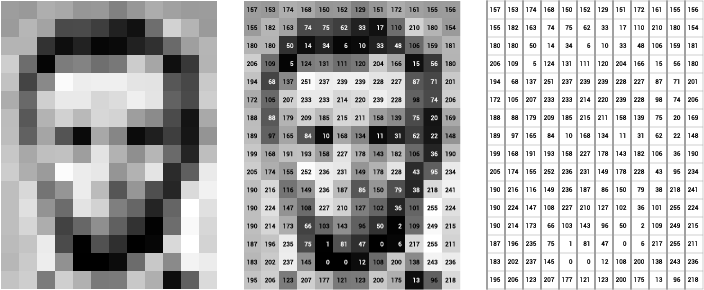
\includegraphics[scale=0.7]{figures/pixel_demo.png}
    \caption{Pixel Demo}
\end{figure}
\\\
\\\

All these values would be in a array for a picture and this is how a picture looks for a computer. Once we give the computer this array of numbers, it will read each pixels and then it will generates probability function that each pixel is more likely to which category for example (.80 for cat, .15 for dog, .05 for bird, etc).
At the end, each pixel will be classified that whether its more likely a cat, dog or a bird.

The part of the program that decides whether a pixel is more likely belong to a dog, a cat or a bird, is called Perceptron in Deep learning terminology. 
\\\

In Deep learning, the Perceptron is an algorithm or a part of Artificial Neural Network which decides whether or not an input, represented by a vector of numbers, belongs to some specific class.
It is a type of linear classifier, i.e. a classification algorithm that makes its predictions based on a linear predictor function combining a set of weights with the feature vector. 


\subsection{Neural network}
Neural networks are a set of algorithms, which are designed to recognize patterns. They read and interpret sensory data through a kind of machine perception, labeling or clustering raw input. The patterns they recognize are numerical, contained in vectors and arrays of three dimensions.

\par A neural network contains layers of interconnected nodes. Each node is a perceptron and is similar to a multiple linear regression. The perceptron feeds the signal which is produced by a multiple linear regression into an activation function that may be nonlinear.

Neural networks help us cluster and classify. Neural Network cam be considered as a clustering and classification layer on top of the raw data stored. They help to group unlabeled data according to similarities among the example inputs and they classify data when they have a labeled dataset to train on. Neural networks can also extract features that are fed to other algorithms for clustering and classification; so deep neural networks can be considered as components of larger machine-learning applications involving algorithms for reinforcement learning classification and regression.



\subsection{Layer}
A layer is a collection of 'nodes' operating together at a specific depth in a neural network.
\newline
Layers can be defined into three types:
\begin{itemize}
    \item \textbf{Input layer}: Contains the raw data or more specifically datasets.
    \item \textbf{Hidden layer(s)}: each layer tries to learn different aspects about the data by minimizing an error/cost function.
    \item \textbf{Output layer}: Is a simple node, which contains the result.
\end{itemize}
\subsection{Nodes}
\par A neural network contains layers of interconnected nodes. Each node is a perceptron and is similar to a multiple linear regression. The perceptron feeds the signal which is produced by a multiple linear regression into an activation function that may be nonlinear.

\subsection{Optimizer function}
Optimization generally is the process of or the selection of a best element (with regard to some criterion) from some set of available alternatives.

\par Optimization algorithms helps us to minimize or maximize an Objective function which is simply a mathematical function dependent on the Model’s internal learnable parameters which are used in computing the target values(Y) from the set of predictors(X) used in the model. For example we call the Weights(W) and the Bias(b) values of the neural network as its internal learnable parameters which are used in computing the output values and are learned and updated in the direction of optimal solution i.e minimizing the Loss by the network’s training process and also play a major role in the training process of the Neural Network Model. \newline 
\textbf{Optimization Algorithm falls in 2 major categories}
\begin{enumerate}
    \item \textbf{First Order Optimization Algorithms} \newline
            These algorithms minimize or maximize a Loss function using its Gradient values with respect to the parameters. Most widely used First order optimization algorithm is Gradient Descent.The First order derivative tells us whether the function is decreasing or increasing at a particular point. 
    \item \textbf{Second Order Optimization Algorithms} \newline
            Second-order methods use the second order derivative which is also called Hessian to minimize or maximize the Loss function.
\end{enumerate}
\subsection{Loss function}
As we have mentioned above, we must learn our network by showing the inputs and the associated output.  Then our network  compute  a  model  and  by  give  this  model  unseen  input,  it  predict  an  output  and  we  tell  it  if  the prediction is correct or not.  It then correct its mistake until it reach a certain level of accuracy fixed by the user.  This is when loss functions appear.
\subsection{Linear Classification}
\par In deep learning(machine learning too) we use linear classification to classify and differentiate a bunch or a group of given data into two part by using their characteristics. \newline

% Train a network

\subsection{Train a network}
The training is one of the most important step for the neural network, it will learn by the input and the outputs that we give to him and update its internal state accordingly, to have the calculated outputs as close as possible from the desired outputs. \newline 
For instance we take a simple example to for better comprehension. There are just one input and one output.
% Table
\begin{table}[h!]
\centering
 \begin{tabular}{|c|c|} 
 \hline
 Input & Desired output \\ [0.7ex] 
 \hline\hline
 0 & 0 \\ 
 1 & 2 \\
 2 & 4 \\
 3 & 6 \\
 4 & 8 \\ [1ex] 
 \hline
 \end{tabular}
\end{table}

\vspace{40mm}
\textbf{The Network Training process is divided into the following steps:}
\begin{enumerate}
    \item \textbf{Model initialization} \newline
        The first step is to start randomly from any where to start the model. Thus a random initialization of the model is required. \newline 
        For our numerical case study, let’s consider the following random initialization: (Model 1): y=3.x. The number 3 here is generated at random. Another random initialization can be: (Model 2): y=5.x, or (Model 3): y=0,5.x.
         
    \item \textbf{Forward propagate} \newline
    The natural step to do after initializing the model at random, is to check its performance. We start from the input we have, we pass them through the network layer and calculate the actual output of the model straightforwardly.

% Table
\begin{table}[h!]
\centering
 \begin{tabular}{|c|c|} 
 \hline
 Input & Actual output of model 1 (y = 3.x) \\ [0.5ex] 
 \hline\hline
 0 & 0 \\ 
 1 & 3 \\
 2 & 6 \\
 3 & 9 \\
 4 & 12 \\ [1ex] 
 \hline
 \end{tabular}
\end{table}



    \item \textbf{Loss function} \newline
    Basically it is a performance metric on how well the NN manages to reach its goal of generating outputs as close as possible to the desired values.
    At this stage, in one hand, we have the actual output of the randomly initialised neural network.
    On the other hand, we have the desired output we would like the network to learn.
    Let’s put them all in the same table.\newline
    As we can see that Actual output is closer to Desired output.
   
% Table
\begin{table}[h!]
\centering
 \begin{tabular}{|c|c|c|c|} 
 \hline
 Input & Actual output & Desired output & Absolute Error \\ [0.5ex] 
 \hline\hline
 0 & 0 & 0 & 0\\ 
 1 & 3 & 2 & 1\\
 2 & 6 & 4 & 2\\
 3 & 9 & 6 & 3\\
 4 & 12 & 8 & 4\\ 
 Total & - & - & 10\\ [1ex] 
 \hline
 \end{tabular}
\end{table}


   \item \textbf{Differentiation} \newline
    In this step we use different optimization technique for example greedy search, genetic algorithm etc to compare which on result is more closer to the desire output. 
    

% Table
\begin{table}[h!]
\centering
 \begin{tabular}{|c|c|c|c|c|c|} 
 \hline
 Input & Output & W=3 & rmse (3) & W=3.0001 & rsme \\ [0.5ex] 
 \hline\hline
 0 & 0 & 0 & 0 & 0 & 0\\ 
 1 & 2 & 3 & 1 & 3.0001 & 1.0002\\
 2 & 4 & 6 & 4 & 6.0002 & 4.0008\\
 3 & 6 & 9 & 9 & 9.0003 & 9.0018\\
 4 & 8 & 12 & 16 & 12.0004 & 16.0032\\
 Total & - & - & 30 & - & 30.006 \\[1ex] 
 \hline
 \end{tabular}
\end{table}
\vspace{20mm}

    \item \textbf{Back-propagation} 
        \par Is a method used in artificial neural networks to calculate a gradient that is needed in the calculation of the weights to be used in the network. BackPropagation is shorthand for "the backward propagation of errors," since an error is computed at the output and distributed backwards throughout the network’s layers. It is commonly used to train deep neural networks.
        \begin{figure}[h1]
             \centering 
             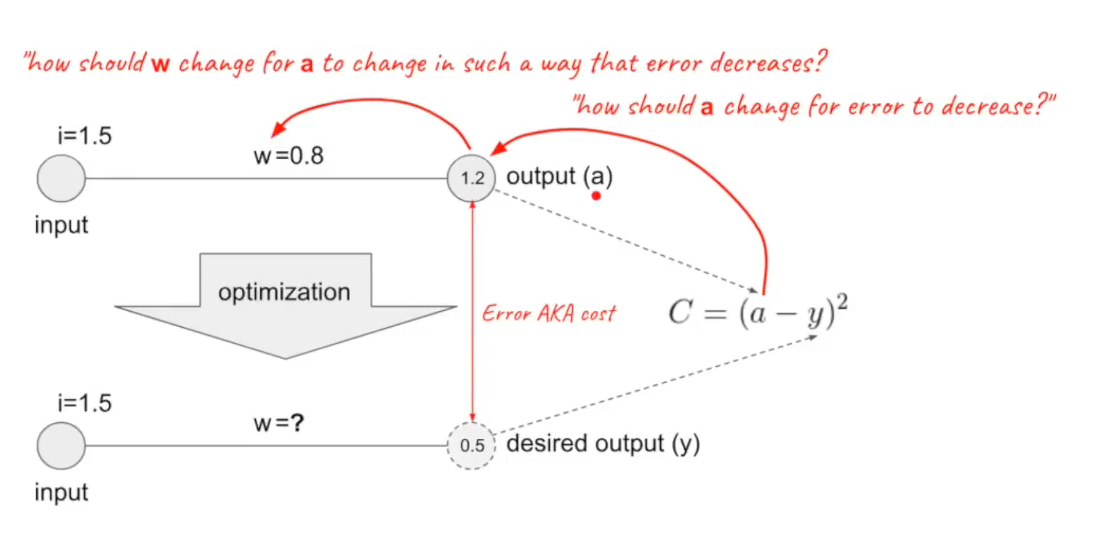
\includegraphics[scale=0.5]{figures/BackProDefine.png}
             \caption{Back Propagation}
        \end{figure} \newline 

        So the Back-propagation process is "how should \textbf{w} change for \textbf{a} to change in such a way that error decreases"?
    \item \textbf{Weight update}
        Weight Update is the process to change the values of weight according to value received from optimization function in order to minimize the cost.
    \item \textbf{Iterate until convergence}
    Since we update the weights, it will take several iterations in order to learn and reach to the almost Desired value. \newline 
    \par \textbf{How many iterations are needed to converge?} \newline 
    
    \par This depends on how strong the learning rate we are applying. High learning rate means faster learning, but with higher chance of instability. \newline 
    It depends as well on the meta-parameters of the network (how many layers, how complex the non-linear functions are). The more it has variables the more it takes time to converge, but the higher precision it can reach. \newline 
    It depends on the optimization method use, some weight updates rule are proven to be faster than others.
    \item \textbf{Overall picture}
\end{enumerate}



\subsection{Evaluate a network}
The network evaluation consist to give to the network inputs, so he can generate using its internal state the most likely output according to its "training experience".

\section{Existing analysis}
We analyzed the existing projects, resources and their interrelated materials. 
\subsection{PyTorch}
PyTorch is an optimized tensor library for deep learning using GPUs and CPUs. In Pytorch, data are represented as tensor or variable.
\subsubsection{Tensor}
Tensor are Python's numpy array but they can be used with GPU for better performance. In our project we will not use the GPU but the CPU, we still working on this feature it will be avaible in newer version of the app. But tensor still useable with CPUs. 
\newline Like arrays, tensors contains elements and can be multidimensional. Frequenntly used tensor are :
\begin{itemize}
    \item Scalar (0-D tensors)
    \item Vector (1-D tensors)
    \item Matrix (2-D tensors)
    \item 3-D tensors
    \item Slicing - tensors
    \item 4-D tensors
    \item 5-D tensors
\end{itemize}

\noindent \emph{torch.rand(10)} returns a tensor filled with 10 random numbers from a uniform distribution on the interval [0, 1)

Image can be represented as 3D-Tensor (height,weight, channel (RGB)) so a 4D-Tensor can be a Tensor with a batch of images. The number of images are represented in the 4th dimension. Slicing tensor are one-dimensional tensor that we slice the elements. For example 1-D\_tensor\textit{[:slice\_index]}   


\subsubsection{Variables}
Pytorch variables can be seen as containers with:
\begin{itemize}
    \item Data : tensor object
    \item Gradients : rate of the change of the loss function
    \item Creator: reference to the function that created it
\end{itemize}

Here is an example on how to create a variable containing a 2x2 tensor:
\begin{lstlisting}
    >> x = Variable(torch.ones(2,2),requires_grad=True)
    >> x.data
    tensor([[1., 1.],
            [1., 1.]])
    >> x.grad
    tensor([[0.2500, 0.2500],
        [0.2500, 0.2500]])
\end{lstlisting}

To compute the actual gradient we must apply the mean() first then the backward() function on x.

\subsection{Computation graphs}
\noindent To represent deep learning algorithms we can use graphs. For a linear relationship model represented as \begin{lstlisting}
    y = wx + b
\end{lstlisting} 
The associated computation graph and its implementation in PyTorch can be:

\subsubsection{Computation graph}
\begin{figure}[!ht]
    \center
    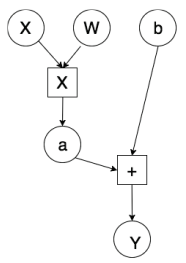
\includegraphics[scale=0.8]{figures/lineasr.png}
    \caption{Linear relationship graph }
\end{figure}

Here, each circle represents a variable. Squared symboles reprensents operators. 

\subsubsection{PyTorch Network implementation}
\begin{lstlisting}
def linear_model(x):
    y = torch.matmul(x,w) 
    return y
\end{lstlisting}

\subsection{Layer}
\subsubsection{Torch.nn}
Torch.nn is a package containing mathematical operations and provides many utilities for efficient seralizing of Tensors.
To build a working deep neural network we must set a collection of 'nodes' operating together in the neural network. 
Pytorch provides a higher level abstraction in torch.nn called layers wich create layer much simpler.
\begin{lstlisting}
CLASS torch.nn.Linear(in_features, out_features, bias=True)
\end{lstlisting}
Applies a linear transformation to the incoming data: y=Ax+b 
\newline
\\
Parameters:

\begin{itemize}
    \item in\_features – size of each input sample
    \item out\_features – size of each output sample
    \item bias – If set to False, the layer will not learn an additive bias. Default: True
\end{itemize}

\noindent The previous model can be represented as a torch.nn layer as follow:
    \begin{lstlisting}
    f = nn.Linear(17,1) 
    \end{lstlisting}
Here a graphical representation of a Convolutional Neural Network 
\subsubsection{Convolution layers}
For an input image as 32x32x3 (3 color channels) if we want to apply a convolution with a filter 5x5x3 (kernel size) we would apply the torch.nn.Conv2d() function

\begin{lstlisting}
CLASS torch.nn.Conv2d(in_channels, out_channels, kernel_size)
\end{lstlisting}

\begin{figure}[!ht]
    \center
    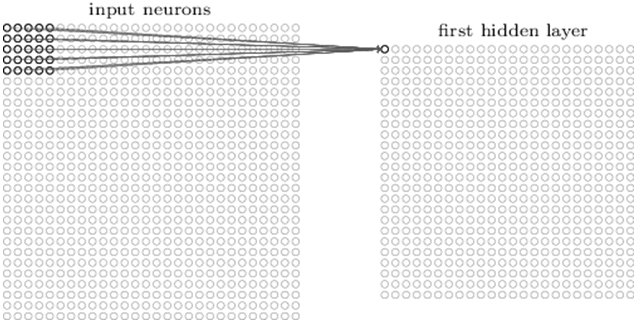
\includegraphics[scale=0.5]{figures/conv2d.png}
    \caption{Visualisation of 5x5 filter producing an activation map}
\end{figure}

More convolution functions in torch.nn:
\begin{itemize}
    \item Conv1d
    \item Conv2d
    \item Conv3d
    \item ConvTranspose1d
    \item ConvTranspose2d
    \item ConvTranspose3d
    \item Unfold
    \item Fold
\end{itemize}




\subsubsection{Pooling layers}
In a CNN, max-pooling, is the most common type of pooling layer used as the next step after convolutional layer. The convolutional layer pass it an input and its work is to reduce the dimensionality of this input. For images, it reduce the number of pixel from the previous convulutional layer. Main goal of this technic is:
\begin{itemize}
    \item By having less spatial information you gain computation performance
    \item Less spatial information also means less parameters, so less chance to over-fit
    \item You get some translation invariance
\end{itemize}

All this technical informations are abstracted in PyTorch. If we want to set an pooling layer we just have to pay attention to some parameters:
\begin{itemize}
    \item Input: H1 x W1 x Depth\_In x N
    \item Stride: Scalar that control the amount of pixels that the window slide.
    \item K: Kernel size
\end{itemize}

PyTorch abstraction :
\begin{lstlisting}
    CLASS torch.nn.MaxPool2d(kernel_size, stride=None)
\end{lstlisting}

All the pooling function in pytorch:
\begin{itemize}
    \item MaxPool1d
    \item MaxPool2d
    \item MaxPool3d
    \item MaxUnpool1d
    \item MaxUnpool2d
    \item MaxUnpool3d
    \item AvgPool1d
    \item AvgPool2d
    \item AvgPool3d
    \item FractionalMaxPool2d
    \item LPPool1d
    \item LPPool2d
    \item AdaptiveMaxPool1d
    \item AdaptiveMaxPool2d
    \item AdaptiveMaxPool3d
    \item AdaptiveAvgPool1d
    \item AdaptiveAvgPool2d
    \item AdaptiveAvgPool3d
\end{itemize}
If user want to use theses functions, they will be listed in a scroll bar in the network edit layer mode.

\subsection{Dropout}
Dropout refers to ignoring neurons during the training phase of certain set of neurons which is chosen at random, the ignored neurons will not be considered during a particular forward or backward pass.
\newline
 At each training stage, individual nodes are either dropped out of the net with probability 1-p or kept with probability p, a smaller network is "created", incoming and outgoing edges to a dropped-out node are removed.
 \newline
 List of all \textbf{Dropout functions}:
 \begin{itemize}
     \item dropout
     \item alpha\_dropout
     \item dropout2d
    \item dropout3d
 \end{itemize}
\subsection{FC Linear}
\subsection{Loss function}
As we say upper, we must learn our network by showing the inputs and the associated output. Then our network compute a model and by give this model unseen input, it predict an output and we tell it if the prediction is correct or not. It then correct its mistake until it reach a certain level of accuracy fixed by the user. This is when loss fuctions appear. Pytorch provide them in torch.nn, As example, the Mean Absolute Error measures the numerical distance between the estimated and actual value. 
\begin{lstlisting}
    CLASS torch.nn.L1Loss(size_average=None, reduce=None, reduction='mean')
\end{lstlisting}


Parameters:	
\begin{itemize}
    \item size\_average (bool, optional) – Deprecated (see reduction). By default, the losses are averaged over each loss element in the batch. Note that for some losses, there multiple elements per sample. If the field size\_average is set to False, the losses are instead summed for each minibatch. Ignored when reduce is False. Default: True
    \item reduce (bool, optional) – Deprecated (see reduction). By default, the losses are averaged or summed over observations for each minibatch depending on size\_average. When reduce is False, returns a loss per batch element instead and ignores size\_average. Default: True
    \item reduction (string, optional) – Specifies the reduction to apply to the output: ‘none’ | ‘mean’ | ‘sum’. ‘none’: no reduction will be applied, ‘mean’: the sum of the output will be divided by the number of elements in the output, "sum": the output will be summed. Note: size\_average and reduce are in the process of being deprecated, and in the meantime, specifying either of those two args will override reduction. Default: "mean"
\end{itemize}

\noindent Here is the list of all the Loss Functions provided by PyTorch:
\begin{itemize}
    \item L1Loss
    \item MSELoss
    \item CrossEntropyLoss
    \item CTCLoss
    \item NLLLoss
    \item PoissonNLLLoss
    \item KLDivLoss
    \item BCELoss
    \item BCEWithLogitsLoss
    \item MarginRankingLoss
    \item HingeEmbeddingLoss
    \item MultiLabelMarginLoss
    \item SmoothL1Loss
    \item SoftMarginLoss
    \item MultiLabelSoftMarginLoss
    \item CosineEmbeddingLoss
    \item MultiMarginLoss
    \item TripletMarginLoss
    
\end{itemize}

\subsection{Optimizer}
Optimizer's goal is to tie together the loss function and model parameters by updating the model into its most accurate possible form by changing the nodes' weight in response to the output of the loss function.

\noindent Here is the list of all the Optimizer Functions provided by Pytorch:
\begin{itemize}
    \item Adadelta
    \item Adagrad
    \item Adam
    \item SparseAdam
    \item Adamax
    \item ASGD
    \item LBFGS
    \item RMSprop
    \item Rprop
    \item SGD
\end{itemize}

\subsubsection{Caffe and Expresso}
To develop our application we think about looking for a existing graphic interface for a deep learning library, Caffe, a deep learning framework already have a graphic interface Expresso but today Caffe's architecture is average.
\newline
Because of the commonalities between Pytorch and Caffe we have decided to inspired our application with Expresso.

\subsubsection{Caffe}
Caffe is a deep learning framework developed by Berkeley AI Research,got an excellent convolutional network implementation used for image processing like image classification, face recognition. Unfortunately it's too cumbersome if we have a big networks compose of many layers.

\subsubsection{Expresso}
Expresso has been developed, to graphically control Caffe library. The framework itself is written in C++, but it has a python interface.

\noindent Expresso is a Python-based graphical user interface made for designing, training, and exploring deep-learning frameworks. It is built atop of Caffe. Its main purpose is to facilitate the use of Caffe by providing a user interface which allow to use most of its features graphically.\\

\noindent Expresso has a handy importing tool which enables users to import different formats of data such as Text, LevelDB, .mat, HDF5 and Folder formats. It provides additional information regarding to the data being imported in a detailed manner.
A technical browser tool is provided, which can be used for a quick preview of the imported data.
The imported data can be exported to the other formats. 

\noindent Another interesting feature is that the back-end framework related to Data view also features a parser. This parser can be utilized to quickly extend the import interface to load data in formats not provided yet in Data view.

\noindent Expresso interface is separated into four different views : Data View, Net View, Train View and Exp View
These different views will basically be our main inspiration for how we organize our application.

\begin{itemize}
    \item Data view allows to import data, by selecting the format of the file. In addition, it provides support for basic data manipulation. The back-end framework of data view also allows to program a new import functionality, which allows to import formats that are not supported yet.
    \item Network view is used to design a deep network from scratch. Each layer of the network can be created and modified using an edit interface, which automatically provides contextual layer description, as the user types. They are color-coded by type, for easy visualization. The "train net" tab allows to create a net, and the "deploy net" tab allows to modify an existing one. All the created networks are Caffe-compatible, which means the user can use them outside of Expresso as well.
    \item The train view is used to train the deep networks. Expresso allows training to be stopped midway, and resumed. In addition to conventional deep network training, it also allows provides support for training external classifiers. These classifiers are trained on features obtained by passing data through trained net.
    \item Experiment view can be used for three important tasks :

    \begin{itemize}
        \item Feature extraction using featuring nets : In the deep-learning field, a "feature" is basically a pattern that can be found in a set of data. For example, it can be used to distinguish shapes in pictures. Feature extraction is a process that consists of finding the features.
        \item Visualizing feature data : This basically allows to visualise the features found in an image, with the use of colors
        \item Testing pre-trained models : Once a model is trained with the use of a training data-set, it can be tested with another data-set. By this process, we can determine the accuracy of a model, which will allow to compare it to other models.
    \end{itemize}
\end{itemize}
The Expresso application is multi-threaded, which means it can enable concurrent execution of tasks. It provides a notification system, which can alert the user when there is an event, or when a task is completed.

%% Mettre les captures d'écran d'expresso
